% ------------------------------------------------------------------
\renewcommand{\thisunit}{MATH327 Unit 4}
\renewcommand{\moddate}{Last modified 27 Feb.~2023}
\setcounter{section}{4}
\setcounter{subsection}{0}
\phantomsection
\addcontentsline{toc}{section}{Unit 4: Ideal gases}
\section*{Unit 4: Ideal gases}
\subsection{\label{sec:regulate}Volume, energy levels, and partition function}
We now apply the canonical ensemble to investigate non-relativistic, classical, ideal gases.
Using statistical physics we will explore how the large-scale behaviours of such gases emerge from the properties of the particles that compose them.
The key particle properties are specified by the adjectives listed above: \\[-24 pt]
\begin{itemize}
  \item \textbf{Classical} systems are those for which we can ignore the effects of quantum mechanics.
        Among other things, this allows us to simultaneously define both the position $(x, y, z)$ and the momentum $\vec p = (p_x, p_y, p_z)$ of each particle with arbitrary precision. % TODO: The `other things' include the possibility of labeling identical particles to distinguish them, which may be too much info to include here...
  \item \textbf{Non-relativistic} particles move with speeds small compared to the speed of light, which allows us to ignore small effects due to special relativity.
        The particles are therefore governed by the laws Isaac Newton published all the way back in 1687.
        In particular, the energy of each particle of mass $m$ is
        \begin{equation*}
          E_n = \frac{1}{2m} p_n^2,
        \end{equation*}
        where $p_n^2 = \vec p_n \cdot \vec p_n = (p_x)_n^2 + (p_y)_n^2 + (p_z)_n^2$ is the inner (or `dot') product of the momentum vector for the $n$th particle in the micro-state of interest.
  \item \textbf{Ideal} gases are those whose constituent particles don't interact with each other.
        As a result, the total energy of the gas is simply the sum of the energies of the $N$ individual particles,
        \begin{equation}
          \label{eq:momentum}
          E = \frac{1}{2m} \sum_{i = n}^N p_n^2.
        \end{equation}
\end{itemize}

As usual for the canonical ensemble, we consider the gas to be in thermodynamic equilibrium, and in thermal contact with a large external thermal reservoir with which it can exchange energy but not particles.
To prevent particle exchange, we can specify that the gas is enclosed in a cubic box with volume $V = L^3$.
The thermal reservoir fixes the temperature $T$ of the gas.

The starting point for our analysis is to compute the partition function
\begin{equation*}
  Z = \sum_i e^{-E_i / T}.
\end{equation*}
Unfortunately there is a challenge confronting this sum over all possible micro-states $\om_i$ of the $N$-particle system.
These micro-states depend on the momenta $\vec{p}_n$ for all $N$ particles, and it's intuitive to suppose that each component of $(p_x, p_y, p_z)_n$ is a continuously varying real number that can (in principle) be distinguished with arbitrary precision.
This implies an uncountably infinite set of distinct momenta and hence an uncountably infinite set of micro-states, making the summation above ill-defined.

To proceed, we need to \textit{regulate} the system so that there are a countable number of micro-states we can sum over to define the partition function.
We do this by positing that the particles' momentum components can take only discrete (or `quantized') values that depend on the volume of the box.
Specifically, we declare that the possible momenta are
\begin{align}
  \label{eq:quant_mom}
  \vec p & = (p_x, p_y, p_z) = \hbar \frac{\pi}{L} (k_x, k_y, k_z) &
  k_{x, y, z} = 0, 1, 2, \cdots.
\end{align}
Each component of the non-negative-integer vector $\vec k = (k_x, k_y, k_z)$ is independent.
The constant factor $\hbar$ (``h-bar''), known as the (reduced) Planck constant (named after \href{https://en.wikipedia.org/wiki/Max_Planck}{Max Planck}), simply converts units from inverse-length ($\frac{1}{L}$) to momentum ($p$).
Very similar discrete momenta turn out to be realized in nature, thanks to quantum mechanics---if you have previously studied quantum physics, you may recognize the momenta for a \href{https://en.wikipedia.org/wiki/Particle_in_a_box}{particle in a box}, but for the purposes of this module we can just adopt this result as an ansatz. % TODO: Planck also introduced this ansatz as a desperate measure; a difference with bona fide quantum mechanics is the presence of a zero mode...

What are the energies that correspond to these discretized momenta?
\begin{mdframed}
  \ \\[60 pt] % WARNING: ADJUSTED SIZE BY HAND TO FILL REMAINDER OF PAGE
\end{mdframed}
You should find energies that fall into discrete \textit{energy levels}, somewhat similar to the spin system considered in \secref{sec:spin_info}.
Unlike the spin system, in this case the energy gaps between subsequent energy levels are not constant.

Even though there are still an infinite number of possible momenta and energy levels for each particle in the gas, these are now countable, making our partition function well-defined.
Let's start by considering the partition function $Z_1$ for a single particle in the box.
The micro-states for this single-particle system are completely specified by that particle's momentum $\vec p$,
\begin{equation*}
  Z_1 = \sum_i \exp\left[-\frac{E_i}{T}\right] = \sum_{\vec p} \exp\left[-\frac{p^2}{2mT}\right] = \sum_{k_{x, y, z} = 0}^{\infty}\exp\left[-\frac{\hbar^2 \pi^2}{2mTL^2}\left(k_x^2 + k_y^2 + k_z^2\right)\right].
\end{equation*}
We can separately sum over each of the independent $(k_x, k_y, k_z)$, and recognize that all three summations are identical:
\begin{align*}
  Z_1 & = \sum_{k_x = 0}^{\infty} \exp\left[-\frac{\hbar^2 \pi^2}{2mTL^2} k_x^2\right] \sum_{k_y = 0}^{\infty} \exp\left[-\frac{\hbar^2 \pi^2}{2mTL^2} k_y^2\right] \sum_{k_z = 0}^{\infty} \exp\left[-\frac{\hbar^2 \pi^2}{2mTL^2} k_z^2\right] \\
      & = \left(\sum_{k_i = 0}^{\infty} \exp\left[-\frac{\hbar^2 \pi^2}{2mTL^2} k_i^2\right]\right)^3.
\end{align*}

For non-relativistic classical gases we can assume that Planck's constant $\hbar$ is extremely small compared to $L\sqrt{mT}$,\footnote{If $m$ is too small, effects due to special relativity become non-negligible.  If $T$ is too small, effects due to quantum physics become non-negligible.  If $L$ is too small, we don't have a sufficiently large-scale (\textit{macroscopic}) system to justify analysis via statistical ensembles in the first place.} so that % TODO: Too-small $L$ also related to quantum effects...
\begin{equation*}
  \frac{\hbar^2 \pi^2}{2mTL^2} \ll 1.
\end{equation*}
This means that the function being summed varies very smoothly as the integer $k_i$ increases, for any $k_i$ small enough to leave the exponential factor non-negligible.
We can therefore accurately approximate each sum by an integral over continuous real $\khat_i$, so that
\begin{equation*}
  \sum_{k_i = 0}^{\infty} \exp\left[-\frac{\hbar^2 \pi^2 k_i^2}{2mTL^2}\right] \approx \int_0^{\infty} d\khat_i \, \exp\left[-\frac{\hbar^2 \pi^2 \khat_i^2}{2mTL^2}\right] = \frac{1}{2} \int_{-\infty}^{\infty} d\khat_i \, \exp\left[-\frac{\hbar^2 \pi^2 \khat_i^2}{2mTL^2}\right].
\end{equation*}
The final equality simply notes that the integrand is an even function of $\khat_i$, as it depends only on $\khat_i^2$.

Since we're back to working with continuous real variables, we may as well use \eq{eq:quant_mom} to return to the original momenta $dp_i = \hbar \frac{\pi}{L} d\khat_i$,
\begin{equation*}
  \sum_{k_i = 0}^{\infty} \exp\left[-\frac{\hbar^2 \pi^2}{2mTL^2} k_i^2\right] = \frac{1}{2} \int \left(\frac{L}{\pi\hbar} dp_i\right) \exp\left[-\frac{p_i^2}{2mT}\right].
\end{equation*}
So we end up with the single-particle partition function
\begin{equation*}
  Z_1 = \left(\frac{L}{2\pi\hbar}\right)^3 \int d^3p \, \exp\left[-\frac{p^2}{2mT}\right],
\end{equation*}
again with $p^2 = p_x^2 + p_y^2 + p_z^2$.
We can now account for all $N$ particles in the ideal gas, which are completely independent and don't interact with each other.
Assuming we can distinguish these particles from each other, then each of them simply contributes an independent factor of $Z_1$ to the overall partition function
\begin{equation}
  \label{eq:ideal_dist_int}
  Z_D = \left(\frac{L}{2\pi\hbar}\right)^{3N} \int d^{3N}p \, \exp\left[-\sum_{n = 1}^N \frac{p_n^2}{2mT}\right],
\end{equation}
where the subscript reminds us of the particles' distinguishability.
We will consider the indistinguishable case below.

We can recognize that each of the $3N$ independent integrations in \eq{eq:ideal_dist_int} is a gaussian integral,
\begin{equation*}
  \frac{L}{2\pi\hbar} \int dp_i \exp\left[-\frac{p_i^2}{2mT}\right] = \frac{L}{2\pi\hbar} \sqrt{2\pi mT} = \sqrt{\frac{mTL^2}{2\pi\hbar^2}} \equiv \frac{L}{\lath(T)}.
\end{equation*}
In the last step we have made the notation more compact by defining the \textit{thermal de~Broglie wavelength} (named after \href{https://en.wikipedia.org/wiki/Louis_de_Broglie}{Louis de Broglie}),
\begin{equation}
  \lath(T) = \sqrt{\frac{2\pi\hbar^2}{mT}}.
\end{equation}
Performing all $3N$ gaussian integrals,
\begin{equation}
  \label{eq:ideal_dist}
  Z_D = \left(\frac{mTL^2}{2\pi\hbar^2}\right)^{3N / 2} = \left(\frac{L}{\lath}\right)^{3N} = \left(\frac{V}{\lath^3}\right)^N,
\end{equation}
since the volume of the box is $V = L^3$.
It is worth emphasizing here that the partition function \emph{depends on the volume of the gas}, in addition to the fixed temperature $T$ and conserved particle number $N$.
This dependence may persist in other quantities derived from the partition function, which we will consider in the next section.

First, let's determine what we would have with indistinguishable particles.
For a classical gas, distinguishability means that we can label the particles and use those labels to tell them apart as they bounce around inside the box.
In the simple two-particle example illustrated below, these labels mean we have a different micro-state $\om_1$ when particle $A$ has momentum $\vec p_1$ while particle $B$ has momentum $\vec p_2$, compared to micro-state $\om_2$ in which particle $A$ has momentum $\vec p_2$ while particle $B$ has momentum $\vec p_1$.
\begin{center}
  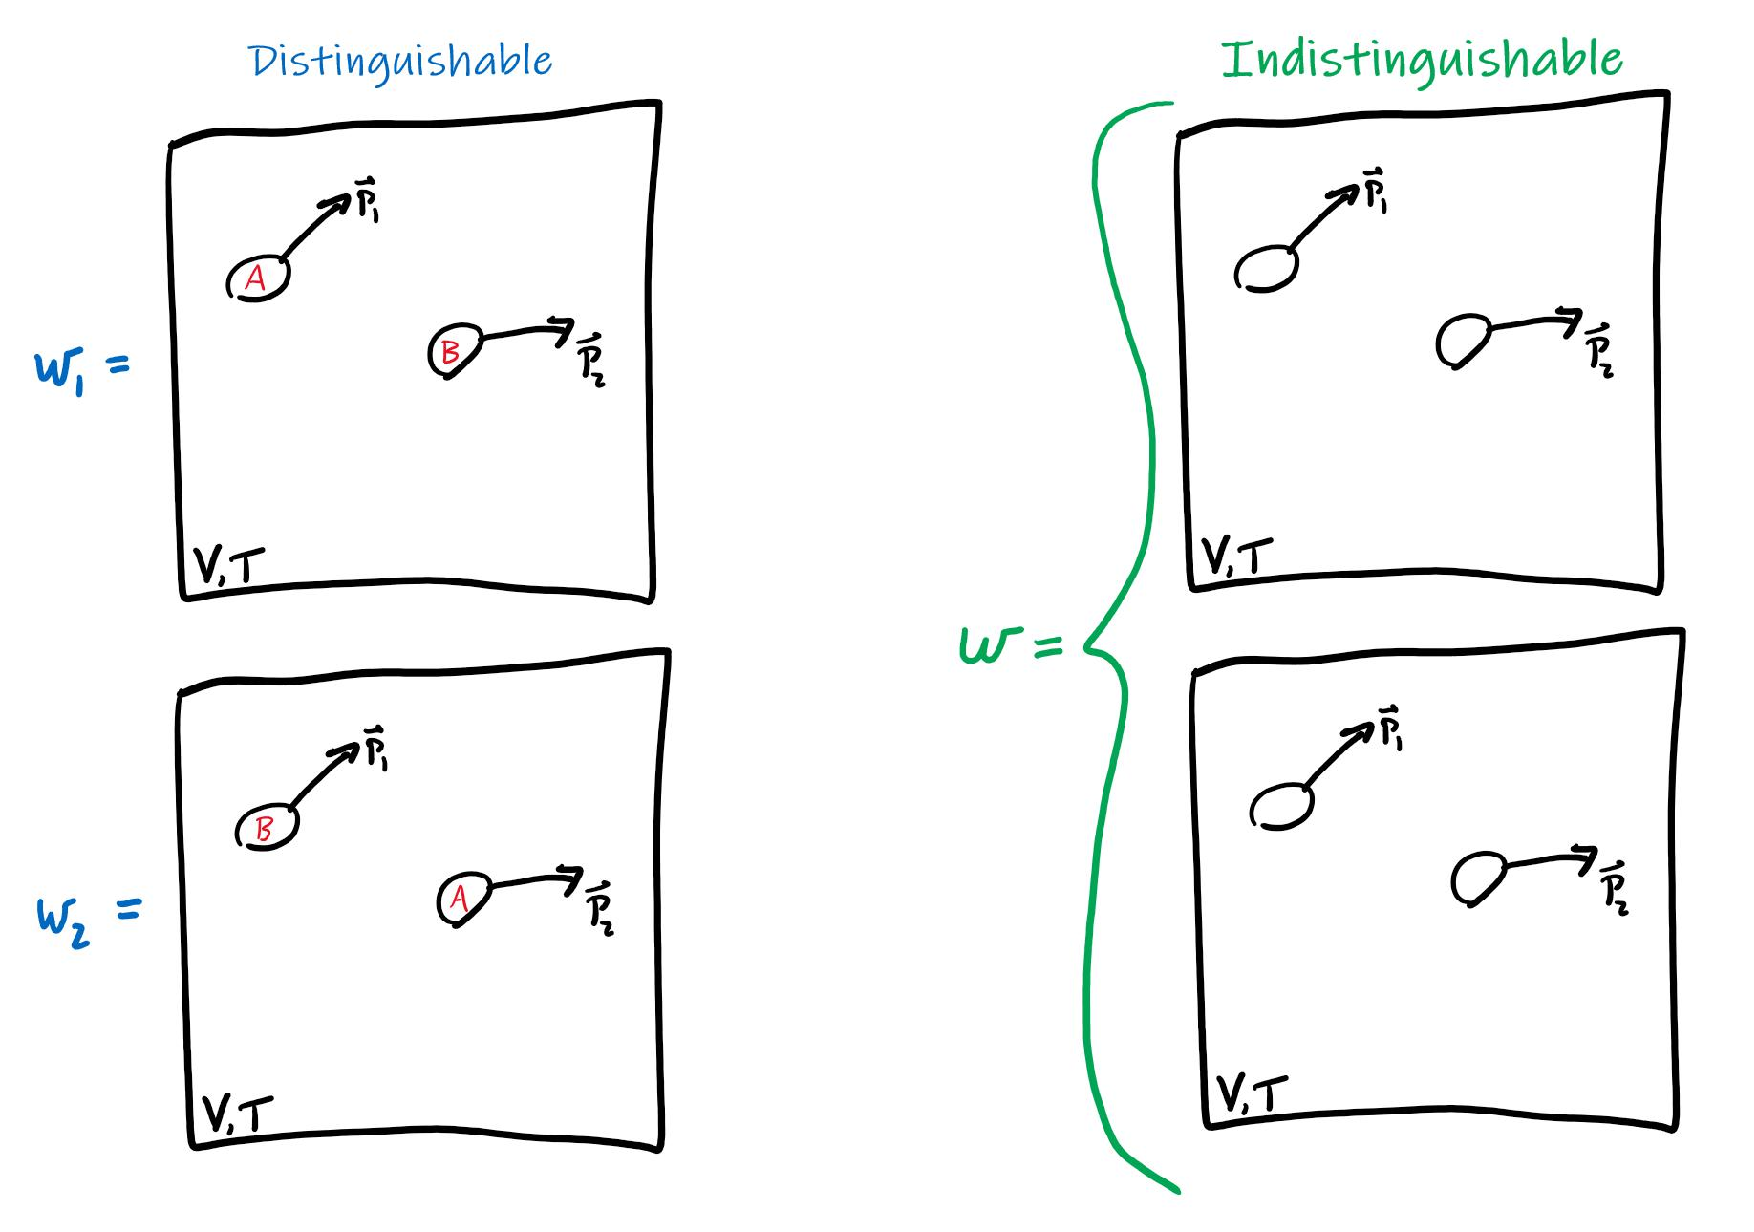
\includegraphics[width=0.7\textwidth]{figs/unit04_distinguish.pdf}
\end{center}
If the particles are indistinguishable, no such labeling is possible, and there is only one micro-state for these $\left\{\vec p_1, \vec p_2\right\}$, rather than two.
This factor of $2$ is not accidental, as you can explore by counting how many micro-states there are for three distinguishable particles with momenta $\left\{\vec p_1, \vec p_2, \vec p_3\right\}$, compared to the single micro-state for the indistinguishable case:
\begin{mdframed}
  \ \\[75 pt] % WARNING: ADJUSTED SIZE BY HAND TO FIT ON PAGE
\end{mdframed}

Generalizing to $N$ particles, we find that ideal gases with distinguishable particles have $N!$ times more micro-states compared to otherwise-identical ideal gases with indistinguishable particles: There are $N$ possible ways to label the particle with momentum $\vec{p}_1$, then $N - 1$ possible labels for $\vec{p}_2$, and so on.\footnote{This argument assumes the momenta themselves are distinguishable, $\vec{p}_i \neq \vec{p}_k$ for any $i \neq k$.  This is a reliable assumption for classical gases with $L\sqrt{mT} \gg \hbar$, but will need to be revisited when we consider quantum statistics.}
The partition function sums over these micro-states, but depends only on their energies, which are independent of any labeling.
Therefore this factor of $N!$ is the only difference between \eq{eq:ideal_dist} and the partition function for indistinguishable particles,
\begin{equation}
  \label{eq:ideal_indis}
  Z_I = \frac{1}{N!} \left(\frac{mTL^2}{2\pi\hbar^2}\right)^{3N / 2} = \frac{1}{N!} \left(\frac{L}{\lath}\right)^{3N} = \frac{1}{N!} \left(\frac{V}{\lath^3}\right)^N.
\end{equation}
% ------------------------------------------------------------------



% ------------------------------------------------------------------
\subsection{Internal energy, and entropy}
Now that we have the canonical partition function, let's apply our work from Unit~3 to predict the large-scale behaviour of the ideal gas it describes.
Our first targets are the average internal energy $\vev{E}$ and entropy $S$ for the gas, as functions of its fixed temperature $T$, conserved particle number $N$, and the volume $V = L^3$ of the box in which it is contained.
Let's begin with the slightly more complicated case of indistinguishable particles, \eq{eq:ideal_indis}.
Recalling the derivatives in Eqs.~\ref{eq:canon_entropy-F}--\ref{eq:canon_energy-F}, we should keep the temperature dependence explicit in our workings, rather than hidden inside the thermal de~Broglie wavelength $\lath(T)$.

Starting by writing down the Helmholtz free energy,
\begin{equation*}
  F_I = -T \log Z_I = -\frac{3NT}{2}\log\left(\frac{mTL^2}{2\pi\hbar^2}\right) + T \log\left(N!\right),
\end{equation*}
we can quickly extract the internal energy,
\begin{equation*}
  \vev{E}_I = -T^2 \pderiv{}{T}\left(\frac{F_I}{T}\right) = -T^2 \pderiv{}{T}\left(-\frac{3N}{2}\log T + T\mbox{-independent}\right) = \frac{3}{2} NT.
\end{equation*}
This in turn provides the entropy
\begin{equation*}
  S_I = \frac{\vev{E}_I - F_I}{T} = \frac{3}{2} N + \frac{3N}{2}\log\left(\frac{mTL^2}{2\pi\hbar^2}\right) - \log\left(N!\right).
\end{equation*}
We can clean this up by reintroducing the thermal de~Broglie wavelength,
\begin{equation*}
  \frac{3N}{2}\log\left(\frac{mTL^2}{2\pi\hbar^2}\right) = \frac{3N}{2}\log\left(\frac{L^2}{\lath^2}\right) = N\log\left(\frac{V}{\lath^3}\right),
\end{equation*}
and by applying Stirling's formula to find
\begin{equation*}
  S_I = \frac{3}{2} N + N\log\left(\frac{V}{\lath^3}\right) - N\log N + N = \frac{5}{2} N + N\log\left(\frac{V}{N\lath^3}\right).
\end{equation*}
We can interpret $N\lath^3$ as the volume `occupied' by the $N$ particles. % TODO: Can revisit when introducing quantum statistics...

\newpage % WARNING: FORMATTING BY HAND
What are the corresponding results for the case of distinguishable particles, where the partition function $Z_D$ is given by \eq{eq:ideal_dist}?
\begin{mdframed}
  $\displaystyle F_D = $ \\[50 pt]
  $\displaystyle \vev{E}_D = $ \\[50 pt]
  $\displaystyle S_D = $ \\[50 pt]
\end{mdframed}
You should find that the energy is insensitive to whether or not we can label the particles:
\begin{equation}
  \label{eq:ideal_energy}
  \vev{E}_D = \vev{E}_I = \frac{3}{2} NT.
\end{equation}
This is in contrast to the spin system we considered in \secref{sec:spin_info}.\footnote{The ultimate origin of this contrast is that each ideal gas micro-state $\om_i$ in the indistinguishable case corresponds to $N!$ micro-states in the distinguishable case, independent of the energy $E_i$.  For the spin system this factor is $\binom{N}{n_+}$ and varies with the energy $E_{n_+}$.}
The entropy, however, does reflect the extra information that distinguishability provides:
\begin{align}
  \label{eq:ideal_entropy}
  S_D & = \frac{3}{2} N + N \log\left(\frac{V}{\lath^3}\right) &
  S_I & = \frac{5}{2} N + N \log\left(\frac{V}{N\lath^3}\right).
\end{align}
Because $N\log N > N$ for $N \gg 1$, we have $S_D > S_I$, as expected.
We can also note that $\lath \to \infty$ as the temperature approaches absolute zero, $T \to 0$, apparently producing negative entropies for fixed $V$.
This is a warning sign that our classical assumptions are breaking down in this regime, and quantum effects would need to be taken into account.
% ------------------------------------------------------------------



% ------------------------------------------------------------------
\subsection{The mixing entropy and the `Gibbs paradox'}
Back in \secref{sec:heat_ex} we considered what would happen if we allowed two micro-canonical systems to exchange energy, and then re-isolated them.
We saw that this procedure obeys the second law of thermodynamics --- the entropy never decreases, though we have to be careful to account for all of the entropy after re-isolating the two systems.

We can now carry out a similar thought experiment of allowing two \emph{canonical} systems to exchange \emph{particles}, and then re-separating them.
We demand that both canonical ensembles are in thermodynamic equilibrium with each other, for instance by sharing the same thermal reservoir with temperature $T$.
This procedure is illustrated below, where we simplify the setup by taking the two initial systems to have equal volumes, $V_A = V_B = V$, and numbers of particles, $N_A = N_B = N$.

\begin{center}
  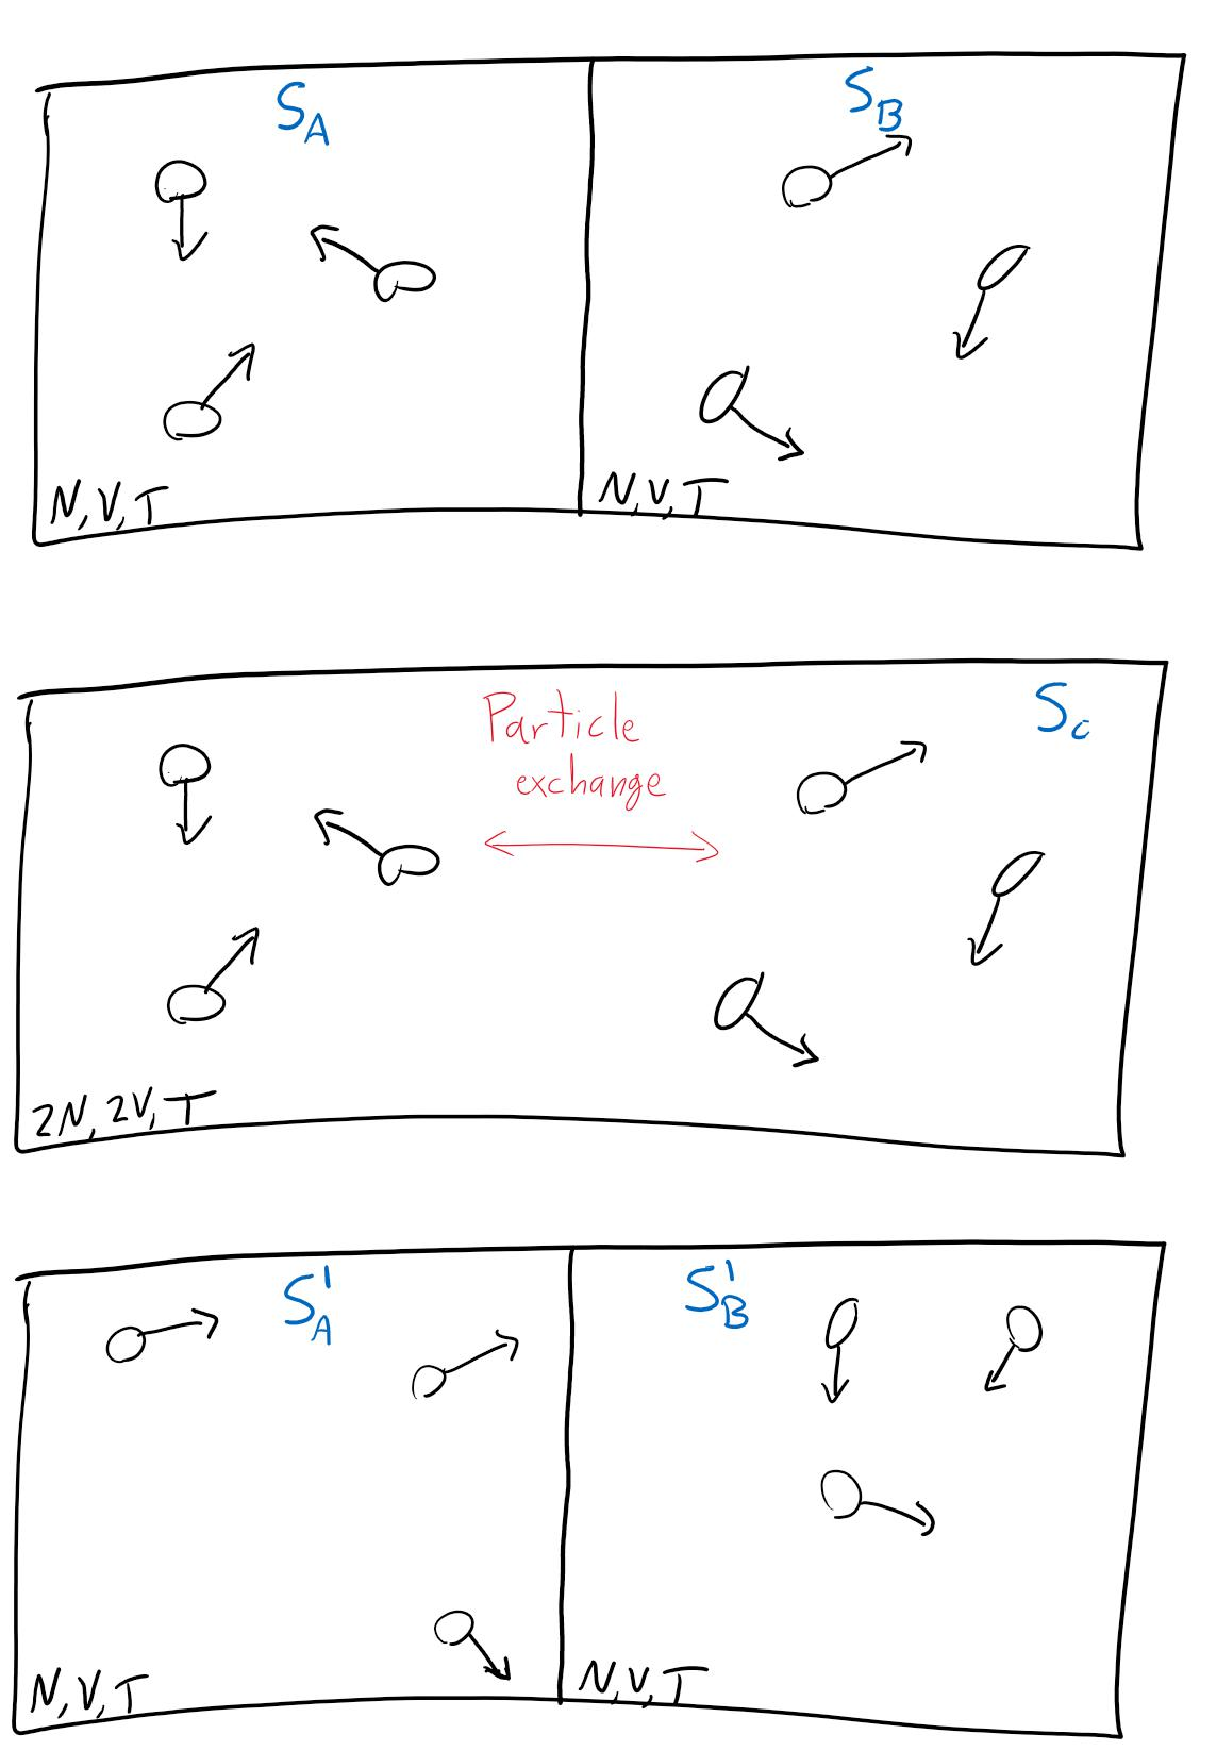
\includegraphics[width=0.7\textwidth]{figs/unit04_mixing.pdf}
\end{center}

We can represent the process of combining and then re-separating these systems by writing
\begin{equation*}
  \Om_A + \Om_B \lra \Om_C \lra \Om_A' + \Om_B'.
\end{equation*}
What is the entropy for each of these three stages?
Since the entropies depend on whether or not the particles in the gas are distinguishable from each other, let's first consider the case of \textit{indistinguishable} particles.

\newpage % WARNING: FORMATTING BY HAND
The initial entropy is the sum of the contributions from the two canonical systems, $S_A + S_B$, both of which are the same thanks to our simplification above, and are given by \eq{eq:ideal_entropy}:
\begin{mdframed}
  $\displaystyle S_A + S_B = $ \\[50 pt]
\end{mdframed}
To find the entropy $S_C$ of the combined system, we just need to consider what happens when we double the volume and also double the number of particles:
\begin{mdframed}
  $\displaystyle S_C = $ \\[50 pt]
\end{mdframed}
You should find $S_C = S_A + S_B$, which is consistent with the second law of thermodynamics.

Things are more complicated when we re-separate the systems.
Analogously to our considerations in \secref{sec:heat_ex}, we need to sum over all the possible ways of dividing the $2N$ indistinguishable particles between the two re-separated boxes.
In particular, we need to perform this sum at the stage of computing the partition function $Z'$ for $\Om_A' + \Om_B'$, since this is the fundamental quantity from which the entropy is then derived as $S = \pderiv{}{T}\left(T\log Z'\right)$. % TODO: In other words, we have the logarithm of a sum rather than a sum of logarithms...
In other words, we have to consider a logarithm of a sum rather than a sum of logarithms.

If $\nu$ particles end up in system $\Om_A'$, then the other system $\Om_B'$ must contain the remaining $2N - \nu$ particles, giving us
\begin{equation*}
  Z_{\nu} = \frac{1}{\nu!} \left(\frac{V}{\lath^3}\right)^{\nu} \times \frac{1}{(2N - \nu)!} \left(\frac{V}{\lath^3}\right)^{2N - \nu} = \frac{1}{\nu! \, (2N - \nu)!} \left(\frac{V}{\lath^3}\right)^{2N}.
\end{equation*}
Summing over all possible values of $0 \leq \nu \leq 2N$,
\begin{align*}
  & Z' = \sum_{\nu = 0}^{2N} Z_{\nu} = \left(\frac{V}{\lath^3}\right)^{2N} \sum_{\nu = 0}^{2N} \frac{1}{\nu! \, (2N - \nu)!} = \left(\frac{V}{\lath^3}\right)^{2N} \frac{1}{(2N)!} \sum_{\nu = 0}^{2N} \binom{2N}{\nu} \cr
  \implies & S_A' + S_B' = 2N \pderiv{}{T}\left(T\log \left[\frac{V}{\lath^3}\right]\right) - \log[(2N)!] + \log\left[\sum_{\nu = 0}^{2N} \binom{2N}{\nu}\right].
\end{align*}
This is a complicated expression.
We can simplify it with an approximation considered by J.\ Willard Gibbs in the 1870s, which we have already motivated in some of our tutorial discussions.
For large $N \gg 1$, we saw that the entropy of two subsystems in thermal contact is nearly saturated by the case in which the energy is divided roughly evenly between the two subsystems, rather than being mostly in one of them.
The same thing happens for two systems that are allowed to exchange particles: there are far more micro-states with particles divided roughly evenly between the two subsystems, $N_A' \approx N_B' \approx N$, compared to the particles being mostly in one of them.

So we declare $N_A' = N_B' = N$, as drawn in the illustration above.
This suffices to establish $\Om_A' = \Om_A$ and $\Om_B' = \Om_B$, producing a final entropy of $S_A' + S_B' = S_A + S_B$ that satisfies the second law of thermodynamics:
\begin{equation*}
  S_A' + S_B' = S_C = S_A + S_B.
\end{equation*}
This is just what we would expect from everyday experience: opening a door between two identical rooms doesn't produce any dramatic effects, nor does reversing that process by closing the door.

Something interesting happens when we repeat this analysis for the case of \textit{distinguishable} particles, using our result for $S_D(N, V)$ in \eq{eq:ideal_entropy}.
If we consider the difference between the combined entropy $S_C$ and the initial entropy $S_A + S_B$,
\begin{align}
  \De S_{\mathrm{mix}} & = S_C - (S_A + S_B) = S_D(2N, 2V) - 2S_D(N, V) \cr
                       & = 3N + 2N \log\left(\frac{2V}{\lath^3}\right) - \left[3N + 2N \log\left(\frac{V}{\lath^3}\right)\right] = 2N\log 2 > 0, \label{eq:mixing_entropy}
\end{align}
we find that the entropy increases upon combining the two initial systems.
This $\De S_{\mathrm{mix}} > 0$ is known as the \textbf{mixing entropy}.

This result $S_C > S_A + S_B$ is what we would expect from the second law of thermodynamics.
However, repeating the argument above---that we should have $N_A' \approx N_B' \approx N$ and therefore $S_A' + S_B' = S_A + S_B$ after re-separating the systems---would imply $S_A' + S_B' < S_C$, indicating a \textit{decrease} in the entropy by $\De S_{\mathrm{mix}}$ and an apparent violation of the second law.
This is known as the `Gibbs paradox', though Gibbs himself explained how a paradox is avoided.

The explanation is that because the particles are now distinguishable, $N_A' = N_A$ no longer suffices to establish $\Om_A' = \Om_A$ and $S_A' = S_A$.
Recovering $\Om_A$ would additionally require that the $N_A'$ particles in the re-separated system are the \emph{same} distinguishable particles that were initially in $\Om_A$.
While we can still expect $N_A' \approx N_B' \approx N$, the vast majority of the resulting micro-states will not correspond to micro-states of $\Om_A$ and $\Om_B$.
Summing over these additional possibilities ensures $S_A' + S_B' > S_A + S_B$, and it turns out $S_A' + S_B' \geq S_C$ as well, obeying the second law of thermodynamics.

These thought experiments provide another example of behaviour that differs depending only on the intrinsic information content of the system --- whether or not the particles in an ideal gas can be distinguished from each other in principle.
Mixing gases of distinguishable particles introduces a positive mixing entropy, \eq{eq:mixing_entropy}, but for gases of indistinguishable particles there is no change in entropy when we let two subsystems mix, or when we reverse that process and re-separate them.
Due to the second law of thermodynamics, processes that produce an increase in entropy are \href{https://en.wikipedia.org/wiki/Irreversible_process}{irreversible}.
% ------------------------------------------------------------------



% ------------------------------------------------------------------
\subsection{\label{sec:ideal_gas}Pressure, ideal gas law, and equations of state}
Below \eq{eq:ideal_dist} we emphasized that the ideal gas partition function depends on the volume of the gas, $V$, in addition to the fixed temperature $T$ and conserved particle number $N$ that always characterize systems governed by the canonical ensemble.
Parameters like $V$ that appear in the partition function are called \textbf{control parameters}, with the idea that they can (in principle) be controlled in experiments.
Control parameters generally enter the partition function through the definition of the energies $E_i$ for the micro-states $\om_i$.
Another example is the magnetic field strength $H$ for the spin systems we considered earlier.

Focusing on ideal gases for now, we see that all dependence on $V$ drops out in our results for the average internal energy, \eq{eq:ideal_energy}.
On the other hand, the entropies in \eq{eq:ideal_entropy} do depend on the volume.
For both cases of distinguishable and indistinguishable particles, the entropy $S$ depends on the same combination of volume and temperature: $V \lath^{-3} \propto V T^{3/2}$.
If we keep $N$ fixed and consider using our experimental control to change the volume and the temperature of the system, the entropy will typically change as a consequence, unless the following relation is satisfied:
\begin{equation*}
  V T^{3/2} = \mbox{constant} \qquad \implies \qquad S = \mbox{constant.}
\end{equation*}

Such \textbf{constant-entropy (or isentropic) processes} will be important in our upcoming analyses of thermodynamic cycles.\footnote{The term \emph{isentropic} is based on the Greek word $\iota\sigma o\varsigma$ (``isos''), meaning ``equal''.}
These cycles will involve making changes to control parameters, which is a topic we have already started to consider through the micro-canonical temperature (\eq{eq:temperature}) and the canonical heat capacity (\eq{eq:heat_cap}).
The pressure of an ideal gas is similarly connected to a change in its volume, which we can motivate by thinking about squeezing an inflated balloon into a small box.

\begin{shaded}
  The \textbf{pressure} is defined to be
  \begin{equation}
    \label{eq:pressure}
    P = -\left. \pderiv{}{V} \vev{E}\right|_S,
  \end{equation}
  with constant entropy $S$.
  In words, the pressure is the isentropic response of the system's internal energy to a change in its volume.
\end{shaded}

In Unit~5 we will look in detail at processes that change some or all of the pressure, volume, temperature, or internal energy of an ideal gas, with $N$ fixed.
Although changing the temperature departs from the assumptions of the canonical ensemble, we will be able to understand such a process as a change from one canonical system (in thermodynamic equilibrium with a thermal reservoir that fixes the initial temperature $T_0$) into another (in thermodynamic equilibrium with a different thermal reservoir that fixes the final temperature $T_f$).

If we consider an isentropic process with $N$ fixed, then the temperature and volume are related,
\begin{equation*}
  V T^{3/2} = c^{3/2} \qquad \lra \qquad T = c V^{-2 / 3},
\end{equation*}
with $c$ a constant.
By inserting this into \eq{eq:ideal_energy}, we can relate the average internal energy to the volume,
\begin{equation*}
  \vev{E} = \frac{3}{2} NT = \frac{3c}{2} N V^{-2 / 3} \qquad \mbox{for constant entropy}.
\end{equation*}
Using this constant-entropy expression, what is the pressure for the ideal gas?
\begin{mdframed}
  $\displaystyle P = -\left. \pderiv{}{V} \vev{E}\right|_S = $ \\[100 pt]
\end{mdframed}

\begin{shaded}
  You should find the \textbf{ideal gas law},
  \begin{equation}
    \label{eq:ideal_gas_law}
    PV = NT,
  \end{equation}
  which is an example of an \textbf{equation of state}.
\end{shaded}

The ``state'' being referred to by this terminology is different from the micro-states that we have mostly discussed up until now.
Whereas each micro-state is defined by detailed information about the microscopic degrees of freedom that constitute the system, this \textbf{thermodynamic state} or \textbf{macro-state} concerns only the large-scale (\textit{macroscopic}) properties of the system, such as its pressure, volume, temperature, or internal energy.
Equations of state are relations between these large-scale properties.

Historically, equations of state were observed empirically and studied experimentally well before the mathematical development of statistical physics.
In the 1660s, for instance, \href{https://en.wikipedia.org/wiki/Robert_Boyle}{Robert Boyle} experimented with changing the pressure of a gas while holding its temperature fixed, finding a special case of the ideal gas law,
\begin{equation*}
  PV = \mbox{constant} \qquad\qquad \mbox{for constant } N \mbox{ and } T,
\end{equation*}
which became known as ``\href{https://en.wikipedia.org/wiki/Boyle's_law}{Boyle's law}''.
(I include the quotation marks to acknowledge the limitations of assigning individuals full credit for advances arising from the work of broad scientific communities.)

\newpage % WARNING: FORMATTING BY HAND
Other equations of state reflecting different aspects of the ideal gas law were uncovered during the Industrial Revolution:
 \\[-24 pt]
\begin{itemize}
  \item $\displaystyle \frac{V}{T} = \mbox{constant}$ \qquad\qquad for constant $N$ and $P$ (1787, ``\href{https://en.wikipedia.org/wiki/Charles's_law}{Charles's law}'') %, attributed to \href{https://en.wikipedia.org/wiki/Jacques_Charles}{Jacques Charles}
  \item $\displaystyle \frac{P}{T} = \mbox{constant}$ \qquad\qquad for constant $N$ and $V$ (1802, ``\href{https://en.wikipedia.org/wiki/Gay-Lussac's_law}{Gay-Lussac's law}'') %, attributed to \href{https://en.wikipedia.org/wiki/Joseph_Louis_Gay-Lussac}{Joseph Gay-Lussac}
  \item $\displaystyle \frac{V}{N} = \mbox{constant}$ \qquad\qquad for constant $P$ and $T$ (1812, ``\href{https://en.wikipedia.org/wiki/Avogadro's_law}{Avogadro's law}'') %, attributed to \href{https://en.wikipedia.org/wiki/Amedeo_Avogadro}{Amedeo Avogadro}
\end{itemize}
In the 1830s \href{https://en.wikipedia.org/wiki/Benoit_Paul_Emile_Clapeyron}{\'Emile Clapeyron} combined these empirical results into the ideal gas law itself, which \href{https://en.wikipedia.org/wiki/August_Kroenig}{August Kr{\"o}nig} and \href{https://en.wikipedia.org/wiki/Rudolf_Clausius}{Rudolf Clausius} independently derived on the basis of statistical physics in the 1850s.
These historical data are useful to illustrate how progress in scientific and mathematical understanding went hand-in-hand with industrial developments, including the design of engines and related machines, which are connected to our next topic of thermodynamic cycles.
% ------------------------------------------------------------------
